% Drafted by moonshotai/kimi-k3.1-pro (Open Math OS worker), 2026-11-13. Not yet human-verified.
\documentclass[aspectratio=169,11pt]{beamer}
\usetheme{default}
\usecolortheme{seahorse}
\setbeamertemplate{navigation symbols}{}
\setbeamertemplate{footline}[frame number]
\setbeamercolor{frametitle}{fg=blue!50!black}
\setbeamercolor{title}{fg=blue!50!black}
\usepackage{amsmath,amssymb}
\usepackage{tikz}
\usetikzlibrary{arrows.meta,positioning}
% colours shared with talk/figures/make_figures.py (symmetric = blue circle, asymmetric = orange square)
\definecolor{symblue}{HTML}{2A78D6}
\definecolor{asymorange}{HTML}{EB6834}
\definecolor{atomgreen}{HTML}{1BAF7A}

% ---- status switches: change these two lines after human sign-off ----
\newcommand{\claimstatus}{candidate proof, under verification}
\newcommand{\ourresult}{Claim}
% --------------------------------------------------------------------
\newcommand{\status}{\par\vfill{\tiny\color{gray}\claimstatus\par}}
\newcommand{\vp}{v_p}
\newcommand{\sd}{s_p}
\newcommand{\Z}{\mathbb{Z}}
\newcommand{\Cq}{C_n^{(q)}}
\DeclareMathOperator{\Fix}{Fix}

\tikzset{
  intnode/.style={circle,draw,fill=black,inner sep=1.4pt},
  symnode/.style={circle,draw=white,fill=symblue,inner sep=2.2pt},
  asymnode/.style={rectangle,draw=white,fill=asymorange,inner sep=2.7pt},
  leafdot/.style={circle,draw,fill=white,inner sep=1.2pt},
  atom/.style={regular polygon,regular polygon sides=3,draw=atomgreen,fill=atomgreen!18,
               inner sep=1pt,minimum size=9mm,font=\small},
  treeedge/.style={draw,thick}
}

\title[Rotations and Fuss--Catalan numbers]%
{The power of $p$ in Fuss--Catalan numbers\\from symmetries of trees}
\subtitle{Caltech Mathathon 2026 --- Problem 137}
\author{Mighty Math Magicians}
\date{15 November 2026}

\usetikzlibrary{shapes.geometric}
\begin{document}

% 1 ------------------------------------------------------------------
\begin{frame}
  \titlepage
  \vspace{-0.5em}
  \centering\footnotesize A counting fact deserves a counting proof.
\end{frame}

% 2 ------------------------------------------------------------------
\begin{frame}{A pattern in the Catalan numbers}
  \begin{columns}[T]
    \column{0.52\textwidth}
      \centering
      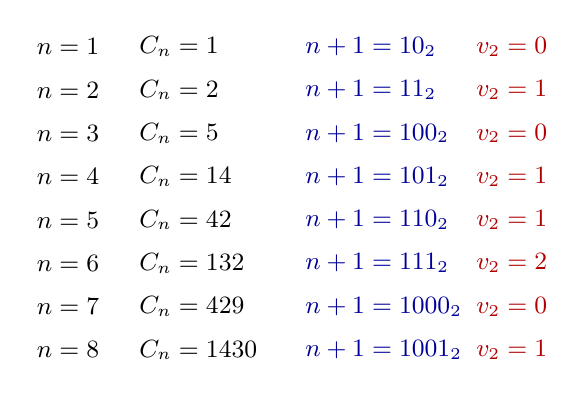
\begin{tikzpicture}[x=0.62cm,y=0.55cm]
        \foreach \x/\n/\c/\b/\e in {
          1/1/1/10/0,
          2/2/2/11/1,
          3/3/5/100/0,
          4/4/14/101/1,
          5/5/42/110/1,
          6/6/132/111/2,
          7/7/429/1000/0,
          8/8/1430/1001/1}
        {
          \node[anchor=west,font=\small] at (0,-\x) {$n=\n$};
          \node[anchor=west,font=\small] at (2.1,-\x) {$C_n=\c$};
          \node[anchor=west,font=\small,blue!60!black] at (5.5,-\x) {$n+1=\b_2$};
          \node[anchor=west,font=\small,red!70!black] at (9.0,-\x) {$v_2=\e$};
        }
      \end{tikzpicture}
    \column{0.44\textwidth}
      \begin{itemize}
        \item $C_n$ counts binary trees with $n$ nodes.
        \item The 2-adic valuation is\\ the number of $1$-bits of $n+1$, minus one.
        \item $C_n$ is \alert{odd} exactly when $n+1$ is a power of $2$.
      \end{itemize}
  \end{columns}
\end{frame}

% 2b (added 2026-11-14 by Claude Fable 5.2; figure: talk/figures/make_figures.py) --------
\begin{frame}{The pattern goes on, for every prime}
  \centering
  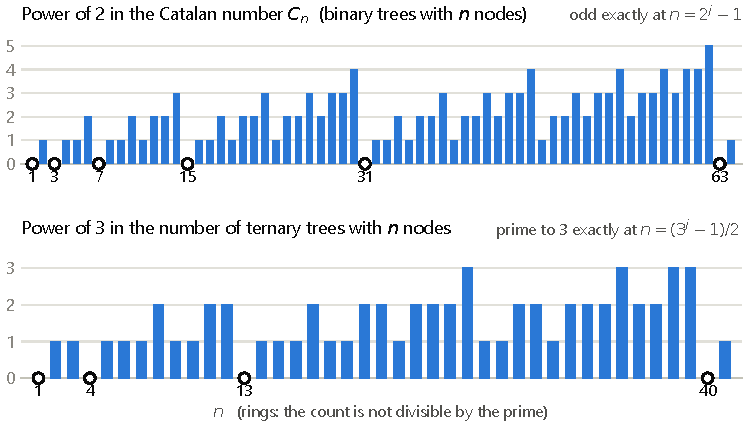
\includegraphics[width=0.76\textwidth]{figures/fig_pattern.pdf}\\[0pt]
  \begin{minipage}{0.93\textwidth}\small
  The power of $p$ is $\bigl(\text{digit sum of the number of leaves in base }p\,-\,1\bigr)/(p-1)$.
  This is known, \emph{by computing with factorials}.
  \textbf{Why should the digits of a number have anything to do with trees?}
  \end{minipage}
\end{frame}

% 3 ------------------------------------------------------------------
\begin{frame}{One tree, four sciences}
  \centering
  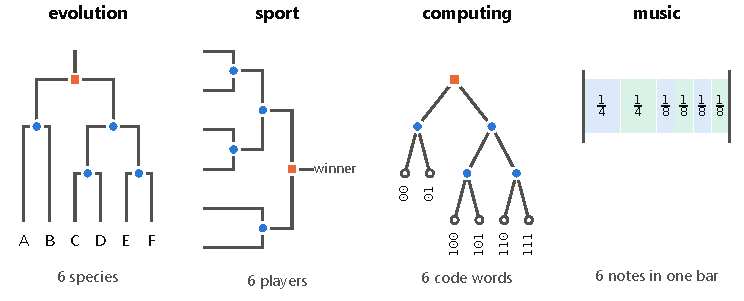
\includegraphics[width=0.88\textwidth]{figures/fig_dialects.pdf}\\[1pt]
  \begin{minipage}{0.96\textwidth}\small
  The left-to-right order of the branches means nothing here: only the \emph{shape} counts.
  \textbf{How many ordered trees stand over one shape? Always a power of $2$.}
  The smallest power that occurs is the power of $2$ in the Catalan number.\\[2pt]
  {\footnotesize $6=110_2$: one node has to be lopsided (orange), and one is enough. Biologists count
  these nodes to measure the balance of an evolutionary tree (Kersting--Fischer 2021).}
  \end{minipage}
\end{frame}

% 3b (added 2026-11-14) ----------------------------------------------
\begin{frame}{Chemistry does it with $p=3$}
  \centering
  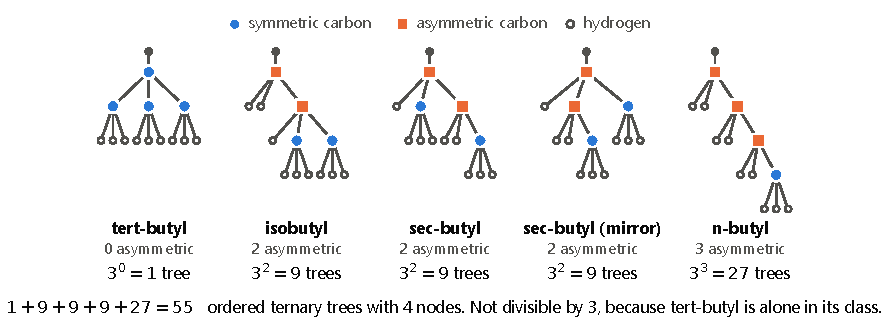
\includegraphics[width=0.96\textwidth]{figures/fig_butyl.pdf}\\[1pt]
  \begin{minipage}{0.96\textwidth}\footnotesize
  The three further bonds of a carbon atom can be \emph{rotated}, not reflected: a cyclic group of
  order $3$ at every node. Ternary trees up to rotation are the alkyl groups, mirror images counted
  separately: $1,1,2,5,11,28,\dots$ (OEIS A000625).
  \end{minipage}
\end{frame}

% 3 ------------------------------------------------------------------
\begin{frame}{The problem}
  A \emph{$q$-ary tree}: every node has $q$ ordered branches,
  each empty or again a $q$-ary tree.
  \[
    \Cq=\frac{1}{(q-1)n+1}\binom{qn}{n},\qquad
    m=(q-1)n+1=\#\text{leaves}.
  \]
  \textbf{Known (Konvalinka 2007, via factorials).}
  For $q=p^k$, $p$ prime,
  \[
    \vp\!\bigl(\Cq\bigr)=\frac{\sd(m)-1}{p-1},
  \]
  where $\sd(m)$ is the sum of the base-$p$ digits of $m$.
  \bigskip

  \textbf{Problem 137.} Prove this \alert{from symmetries of trees},
  \emph{without factorial valuations}.
\end{frame}

% 4 ------------------------------------------------------------------
\begin{frame}{Konvalinka's symmetries \dots\ and ours}
  \begin{columns}[T]
    \column{0.48\textwidth}
      \centering\textbf{All permutations}\\[2pt]
      {\small Konvalinka 2007}\\[6pt]
      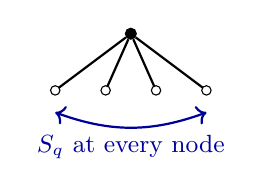
\begin{tikzpicture}[scale=0.8]
        \node[intnode] (r) at (0,0) {};
        \foreach \x/\l in {-1.2/1,-0.4/2,0.4/3,1.2/4}{
          \draw[treeedge] (r) -- (\x,-0.9);
          \node[leafdot] at (\x,-0.9) {};
        }
        \draw[<->,blue!60!black,thick] (-1.2,-1.25) to[bend right=20] (1.2,-1.25);
        \node[blue!60!black,font=\small] at (0,-1.8) {$S_q$ at every node};
      \end{tikzpicture}\\[4pt]
      orbit sizes = products of\\ \textbf{multinomial coefficients}
      \begin{itemize}\small
        \item gives divisibility $p^t\mid\Cq$;
        \item exactness still quoted from factorials.
      \end{itemize}
    \column{0.48\textwidth}
      \centering\textbf{Only rotations}\\[2pt]
      {\small our change}\\[6pt]
      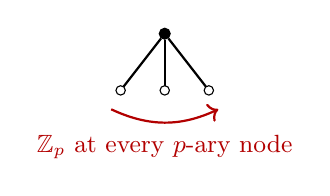
\begin{tikzpicture}[scale=0.8]
        \node[intnode] (r) at (0,0) {};
        \foreach \x in {-0.7,0,0.7}{
          \draw[treeedge] (r) -- (\x,-0.9);
          \node[leafdot] at (\x,-0.9) {};
        }
        \draw[->,red!70!black,thick] (-0.85,-1.2) to[bend right=25] (0.85,-1.2);
        \node[red!70!black,font=\small] at (0,-1.8) {$\Z_p$ at every $p$-ary node};
      \end{tikzpicture}\\[4pt]
      orbit sizes = \textbf{powers of $p$}
      \begin{itemize}\small
        \item a $p$-group (Sylow $p$-subgroup of $S_q$);
        \item minimal orbits can be listed and counted $\bmod\,p$.
      \end{itemize}
  \end{columns}
  \status
\end{frame}

% 5b (added 2026-11-14) ----------------------------------------------
\begin{frame}{Why the smaller group works: bits, not bytes}
  \centering
  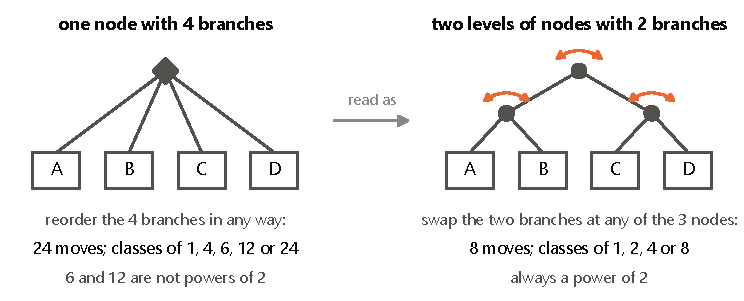
\includegraphics[width=0.9\textwidth]{figures/fig_bits.pdf}\\[5pt]
  \begin{minipage}{0.93\textwidth}\small
  For $q=p^k$: read every $q$-ary node as $k$ levels of $p$-ary nodes, and only \emph{rotate} at each of them.
  Then every class of trees has $p^{d}$ members, where $d$ is the number of asymmetric nodes.
  \end{minipage}
\end{frame}

% 5 ------------------------------------------------------------------
\begin{frame}{Step 0: a $q$-ary tree is a $p$-ary tree}
  \begin{columns}[T]
    \column{0.46\textwidth}
      \centering
      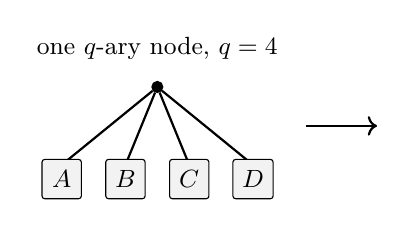
\begin{tikzpicture}[scale=0.9]
        % q-ary node (q=4) and its p-ary block (p=2,k=2)
        \node[intnode] (r) at (0,0) {};
        \foreach \x/\c in {-1.35/A,-0.45/B,0.45/C,1.35/D}{
          \draw[treeedge] (r) -- (\x,-1.1);
          \node[draw,rounded corners=1pt,fill=gray!10,minimum size=5mm,font=\small]
            at (\x,-1.3) {$\c$};
        }
        \node[font=\small] at (0,0.55) {one $q$-ary node, $q=4$};
        \draw[->,thick] (2.1,-0.55) -- (3.1,-0.55);
      \end{tikzpicture}
    \column{0.5\textwidth}
      \centering
      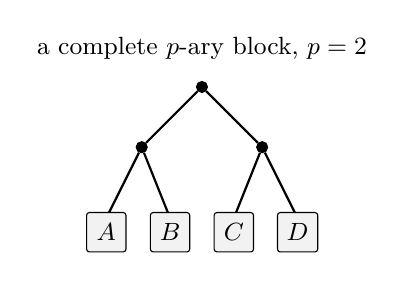
\begin{tikzpicture}[scale=0.9]
        \node[intnode] (r) at (0,0) {};
        \node[intnode] (l) at (-0.85,-0.85) {};
        \node[intnode] (rr) at (0.85,-0.85) {};
        \draw[treeedge] (r) -- (l); \draw[treeedge] (r) -- (rr);
        \foreach \p/\x/\c in {l/-1.35/A,l/-0.45/B,rr/0.45/C,rr/1.35/D}{
          \draw[treeedge] (\p) -- (\x,-1.85);
          \node[draw,rounded corners=1pt,fill=gray!10,minimum size=5mm,font=\small]
            at (\x,-2.05) {$\c$};
        }
        \node[font=\small] at (0,0.55) {a complete $p$-ary block, $p=2$};
      \end{tikzpicture}
  \end{columns}
  \bigskip
  Replace each node by a complete $p$-ary tree of height $k$ ($p^k=q$ branches).
  \begin{itemize}
    \item Bijection: $q$-ary trees $\longleftrightarrow$ $p$-ary trees
          whose leaves all sit at \alert{depth divisible by $k$}.
    \item Leaf count unchanged: $m=(q-1)n+1$.
    \item The answer can only depend on $m$.
  \end{itemize}
\end{frame}

% 6 ------------------------------------------------------------------
\begin{frame}{Step 1: rotate, don't permute}
  \begin{columns}[T]
    \column{0.55\textwidth}
      \centering
      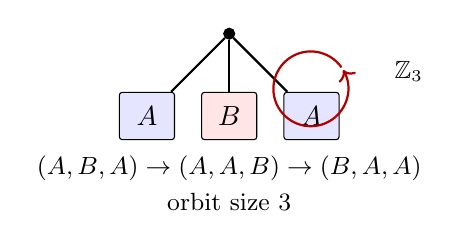
\begin{tikzpicture}[scale=0.95]
        \node[intnode] (r) at (0,0) {};
        \node[draw,rounded corners=1pt,fill=blue!10,minimum width=7mm,minimum height=6mm] (a) at (-1.1,-1.1) {$A$};
        \node[draw,rounded corners=1pt,fill=red!10,minimum width=7mm,minimum height=6mm] (b) at (0,-1.1) {$B$};
        \node[draw,rounded corners=1pt,fill=blue!10,minimum width=7mm,minimum height=6mm] (c) at (1.1,-1.1) {$A$};
        \draw[treeedge] (r) -- (a); \draw[treeedge] (r) -- (b); \draw[treeedge] (r) -- (c);
        \draw[->,thick,red!70!black] (1.5,-0.45) arc[start angle=35,end angle=390,radius=0.5];
        \node[font=\small] at (2.4,-0.5) {$\Z_3$};
        \node[font=\small,align=center] at (0,-2.0)
          {$(A,B,A)\to(A,A,B)\to(B,A,A)$\\[2pt] orbit size $3$};
      \end{tikzpicture}
    \column{0.41\textwidth}
      At each node, cyclically rotate the $p$ subtrees.
      \begin{itemize}
        \item Generates a $p$-group.
        \item Rotations preserve leaf depths, so the class condition survives.
        \item $\sim$ = equivalence generated by these moves.
      \end{itemize}
  \end{columns}
  \bigskip
  \begin{block}{Key definition}
    A node is \textcolor{blue!60!black}{\textbf{symmetric}} if its $p$ subtrees
    are pairwise equivalent, \textcolor{red!70!black}{\textbf{asymmetric}} otherwise.\\
    $d(T)=\#\{$asymmetric nodes of $T\}$.
  \end{block}
\end{frame}

% 7 ------------------------------------------------------------------
\begin{frame}{Class size $=p^{d(T)}$}
  \centering
  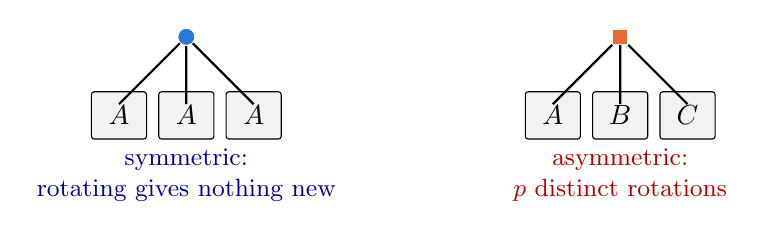
\begin{tikzpicture}[scale=0.95]
    % symmetric node (blue)
    \node[symnode] (s) at (-3.2,0) {};
    \node[draw,rounded corners=1pt,fill=gray!10,minimum width=7mm,minimum height=6mm] at (-4.1,-1.05) {$A$};
    \node[draw,rounded corners=1pt,fill=gray!10,minimum width=7mm,minimum height=6mm] at (-3.2,-1.05) {$A$};
    \node[draw,rounded corners=1pt,fill=gray!10,minimum width=7mm,minimum height=6mm] at (-2.3,-1.05) {$A$};
    \draw[treeedge] (s) -- (-4.1,-0.9); \draw[treeedge] (s) -- (-3.2,-0.9); \draw[treeedge] (s) -- (-2.3,-0.9);
    \node[blue!60!black,font=\small,align=center] at (-3.2,-1.85) {symmetric:\\rotating gives nothing new};
    % asymmetric node (red)
    \node[asymnode] (a) at (2.6,0) {};
    \node[draw,rounded corners=1pt,fill=gray!10,minimum width=7mm,minimum height=6mm] at (1.7,-1.05) {$A$};
    \node[draw,rounded corners=1pt,fill=gray!10,minimum width=7mm,minimum height=6mm] at (2.6,-1.05) {$B$};
    \node[draw,rounded corners=1pt,fill=gray!10,minimum width=7mm,minimum height=6mm] at (3.5,-1.05) {$C$};
    \draw[treeedge] (a) -- (1.7,-0.9); \draw[treeedge] (a) -- (2.6,-0.9); \draw[treeedge] (a) -- (3.5,-0.9);
    \node[red!70!black,font=\small,align=center] at (2.6,-1.85) {asymmetric:\\$p$ distinct rotations};
  \end{tikzpicture}
  \bigskip

  \begin{block}{\ourresult\ (class size)}
    $|[T]|=p^{d(T)}$, by induction: the $p$ rotations of a word of length $p$
    are all equal or pairwise distinct, because $p$ is prime.
  \end{block}
  \[
    \Cq=\sum_{\text{rotation classes}}p^{\,d}
    \;\Longrightarrow\;
    \vp(\Cq)\ge \min d,\qquad
    \Cq/p^{\min d}\equiv N_{\min}\pmod p .
  \]
  \status
\end{frame}

% 8 ------------------------------------------------------------------
\begin{frame}{Step 2: every class has at least $p^t$ trees}
  \begin{block}{\ourresult\ (lower bound)}
    Every $p$-ary tree $T$ with $m$ leaves has
    \[
      d(T)\ \ge\ t:=\frac{\sd(m)-1}{p-1}.
    \]
  \end{block}
  Only two digit facts, \textbf{no factorials}:
  \[
    \sd(pa)=\sd(a),\qquad
    \sd(a+b)\le\sd(a)+\sd(b)\ \text{(equality: no carries)}.
  \]
  Induction on $T=(T_1,\dots,T_p)$, $m_i$ leaves in $T_i$:
  \begin{itemize}
    \item \textcolor{blue!60!black}{Symmetric root}: all $m_i$ equal, $m=pm_1$, and
          $d=p\,d(T_1)\ge p\,t(m_1)\ge t(m)$.
    \item \textcolor{red!70!black}{Asymmetric root}:
          $d=1+\sum_i d(T_i)\ge 1+\sum_i t(m_i)\ge t(m)$.
  \end{itemize}
  Hence $p^t\mid\Cq$: Konvalinka's divisibility, now a five-line induction.
\end{frame}

% 8b (optional; added 2026-11-14 by Claude Fable 5.2: the same step, said with carries) ----
\begin{frame}{Step 2 again: the carry budget \hfill\normalsize\textcolor{red!70!black}{same statement, a second way to see it}}
  \centering
  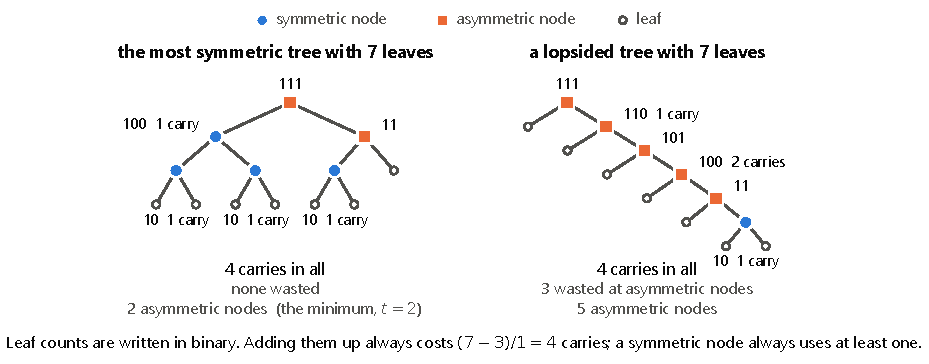
\includegraphics[width=0.92\textwidth]{figures/fig_carry_budget.pdf}\\[2pt]
  \begin{minipage}{0.96\textwidth}\small
  A carry is one trade of $p$ units for $1$ unit in the next column. \textbf{Every} tree with $m$ leaves
  makes $\nu(m)=\frac{m-\sd(m)}{p-1}$ of them. A symmetric node always makes at least one. So at most
  $\nu(m)$ of the $\frac{m-1}{p-1}$ nodes are symmetric: $d(T)\ge\frac{m-1}{p-1}-\nu(m)=t$.
  Equality: no carry is wasted. That is Step~3.
  \end{minipage}
  \status
\end{frame}

% 9 ------------------------------------------------------------------
\begin{frame}{Step 3: minimal trees are built from the digits of $m$}
  \textbf{Minimal} means $d(T)=t$: the smallest classes, size $p^t$.
  \bigskip

  Tracing equality through the induction forces:
  \begin{itemize}
    \item every internal node \textcolor{red!70!black}{asymmetric}
          (the \emph{skeleton}, $t$ nodes);
    \item hanging from it, \textbf{complete trees} of height $j$ --- \emph{atoms};
    \item \alert{no carries} at every node $\Rightarrow$
          exactly $m_j$ atoms of height $j$:\\
          \centering\textbf{the atoms are the base-$p$ digits of $m$.}
  \end{itemize}
  \bigskip
  \begin{block}{\ourresult\ (skeleton bijection)}
    Minimal classes $\longleftrightarrow$ cyclic skeleton trees on the digit atoms,
    an atom of height $j$ sitting at depth $\equiv -j \pmod k$.
  \end{block}
  \status
\end{frame}

% 9b (added 2026-11-14) ----------------------------------------------
\begin{frame}{The answer in one picture}
  \centering
  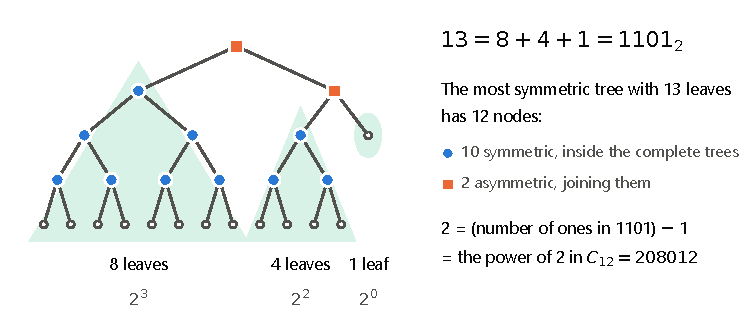
\includegraphics[width=0.93\textwidth]{figures/fig_atoms.pdf}\\[3pt]
  \begin{minipage}{0.93\textwidth}\small
  The most symmetric tree is made of complete trees, one for each digit of $m$.
  The digits are not a formula here: \textbf{they are the building blocks.}
  \end{minipage}
  \status
\end{frame}

% 10 -----------------------------------------------------------------
\begin{frame}{Running example: $p=2$, $n=6$}
  \[
    C_6=132=2^2\cdot 33,\qquad m=7=111_2,\qquad t=2 .
  \]
  Atoms of heights $0,1,2$: triangles with $1,2,4$ leaves.
  The three minimal skeletons (unordered binary trees on the atoms):
  \begin{center}
  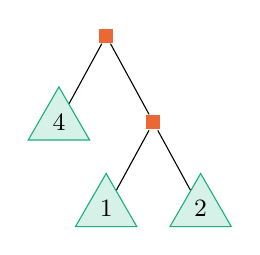
\begin{tikzpicture}[level distance=11mm,sibling distance=12mm]
    \node[asymnode]{}
      child{node[atom]{4}}
      child{node[asymnode]{}
        child{node[atom]{1}} child{node[atom]{2}}};
  \end{tikzpicture}
  \qquad
  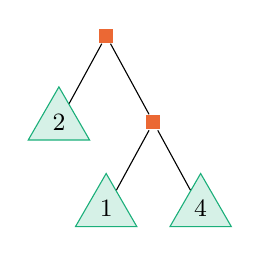
\begin{tikzpicture}[level distance=11mm,sibling distance=12mm]
    \node[asymnode]{}
      child{node[atom]{2}}
      child{node[asymnode]{}
        child{node[atom]{1}} child{node[atom]{4}}};
  \end{tikzpicture}
  \qquad
  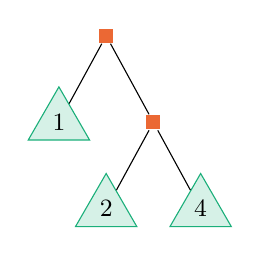
\begin{tikzpicture}[level distance=11mm,sibling distance=12mm]
    \node[asymnode]{}
      child{node[atom]{1}}
      child{node[asymnode]{}
        child{node[atom]{2}} child{node[atom]{4}}};
  \end{tikzpicture}
  \end{center}
  \begin{itemize}
    \item Each class has $2^2=4$ trees; together $132=4\cdot 33$.
    \item $11$ rotation classes in all, $N_{\min}=3$ (odd).
    \item These are the rooted phylogenetic trees on the three $1$-bits of $7$.
  \end{itemize}
  \status
\end{frame}

% 11 -----------------------------------------------------------------
\begin{frame}{Step 4: a carry is a collapsing cherry}
  Count minimal classes $\bmod\,p$ by cycling $p$ same-class labels:
  only \textbf{fixed} trees survive $\bmod\,p$ --- and those have a \emph{cherry}.
  \begin{center}
  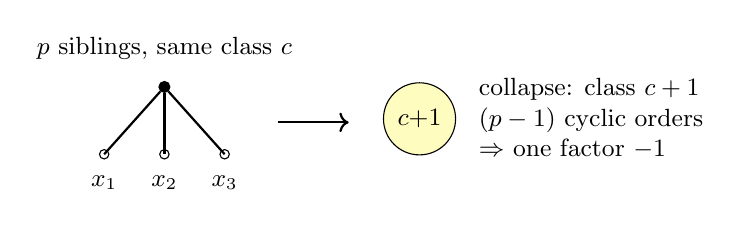
\begin{tikzpicture}[scale=0.9]
    % cherry -> single atom
    \node[intnode] (v) at (0,0) {};
    \foreach \x/\l in {-0.85/x_1,0/x_2,0.85/x_3}{
      \node[leafdot] at (\x,-0.95) {};
      \node[font=\small] at (\x,-1.35) {$\l$};
      \draw[treeedge] (v) -- (\x,-0.95);
    }
    \node[font=\small] at (0,0.55) {$p$ siblings, same class $c$};
    \draw[->,thick] (1.6,-0.5) -- (2.6,-0.5);
    \node[draw,circle,fill=yellow!25,minimum size=6mm,font=\small] at (3.6,-0.45) {$c{+}1$};
    \node[font=\small,align=left,anchor=west] at (4.3,-0.45) {collapse: class $c+1$\\
      $(p-1)$ cyclic orders\\ $\Rightarrow$ one factor $-1$};
  \end{tikzpicture}
  \qquad
  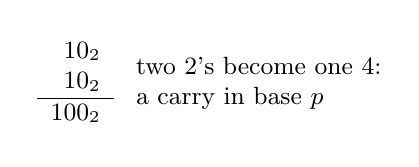
\begin{tikzpicture}[scale=0.75]
    % column addition 2+2 = 4
    \node[font=\small] at (0,0) {$\begin{array}{r}10_2\\10_2\\ \hline 100_2\end{array}$};
    \node[font=\small,align=left] at (3.1,0) {two $2$'s become one $4$:\\
      a \alert{carry} in base $p$};
  \end{tikzpicture}
  \end{center}
  \[
    T(a)\equiv -T(a-p\,e_c+e_{c+1})\pmod p,\qquad
    \text{carries end at one leaf}\;\Rightarrow\;T(a)\equiv(-1)^t .
  \]
  Running example: $T(3)\equiv -T(2)\equiv T(1)=1$, and indeed $T(3)=3$.
  \status
\end{frame}

% 12 -----------------------------------------------------------------
\begin{frame}{Conclusion: exact valuation, plus the residue}
  \begin{block}{\ourresult\ (main statement)}
    For every prime power $q=p^k$,
    \[
      \vp\!\bigl(\Cq\bigr)=\frac{\sd(m)-1}{p-1},
      \qquad m=(q-1)n+1,
    \]
    and, writing $m=\sum_j m_jp^j$ in base $p$,
    \[
      \frac{\Cq}{p^t}\equiv\frac{(-1)^t}{\prod_j m_j!}\pmod p .
    \]
  \end{block}
  \begin{itemize}
    \item Class sizes $p^d$ with $d\ge t$; the sum $\bmod\,p$ sees only minimal classes.
    \item Their number is $\equiv(-1)^t/\prod_j m_j!\not\equiv 0\pmod p$.
    \item No valuation of a factorial, binomial or multinomial is used.
  \end{itemize}
  \status
\end{frame}

% 13 -----------------------------------------------------------------
\begin{frame}{A prime-power example: $p=2$, $q=4$, $n=4$}
  \[
    C_4^{(4)}=140=2^2\cdot 35,\qquad m=13=1101_2,\qquad t=2 .
  \]
  Atoms of heights $0,2,3$ (sizes $1,4,8$); leaf depths must be \textbf{even}
  ($k=2$). Only one skeleton fits:
  \begin{center}
  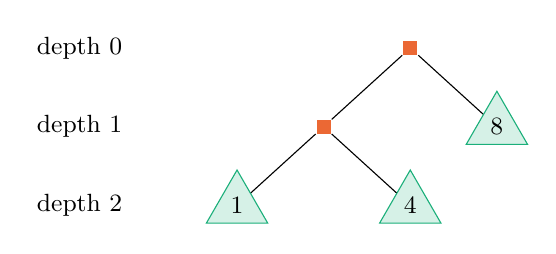
\begin{tikzpicture}[level distance=10mm,sibling distance=22mm]
    \node[asymnode]{}
      child{node[asymnode]{}
        child{node[atom]{1}} child{node[atom]{4}}}
      child{node[atom]{8}};
    \node[font=\small] at (-4.2,0) {depth $0$};
    \node[font=\small] at (-4.2,-1.0) {depth $1$};
    \node[font=\small] at (-4.2,-2.0) {depth $2$};
  \end{tikzpicture}
  \end{center}
  \begin{itemize}
    \item Atom $8$ (height $3$) at depth $1$; atoms $1$, $4$ (heights $0$, $2$) at depth $2$:
          height $+$ depth is even each time.
    \item Carries: $(2,1)\to(0,2)\to(1,0)$, two carries, sign $+1$.
          So $N_{\min}=1$, and indeed $140/4=35$ is odd.
  \end{itemize}
  \status
\end{frame}

% 14 -----------------------------------------------------------------
\begin{frame}{What else falls out \hfill\normalsize\textcolor{red!70!black}{checked numerically, not yet proved}}
  \begin{itemize}
    \item \textbf{Weighted Fuss--Catalan numbers.}
      Konvalinka's weighted theorem seems to need only transitivity on the $q$
      branches; our rotation group is transitive, so the weighted theorem should
      also become free of factorial valuations.
      \par\hfill{\small(conjecture C9)}
    \item \textbf{Level profiles.}
      Rotations preserve the number $n_i$ of nodes at each depth, so $p^t$ should
      divide $\prod_i\binom{q n_i}{n_{i+1}}$ for every profile with $\sum n_i=n$.
      \par\hfill{\small(conjecture C10)}
    \item \textbf{Any closed family.}
      For any rotation-closed family $F$ of trees with $m$ leaves:
      $p^t\mid|F|$ and $|F|/p^t\equiv\#\{\text{minimal classes in }F\}\pmod p$.
      \par\hfill{\small(conjecture C11)}
  \end{itemize}
  \vfill
  {\small Checked by computer: every level profile up to $22$ nodes for $q=2$ (up to
  $12$--$15$ for $q=3,4,5,8,9$); weighted numbers for six values of $q$.
  Not claimed as theorems today.}
\end{frame}

% 14b ----------------------------------------------------------------
\begin{frame}{Why the most symmetric shapes decide}
  \centering
  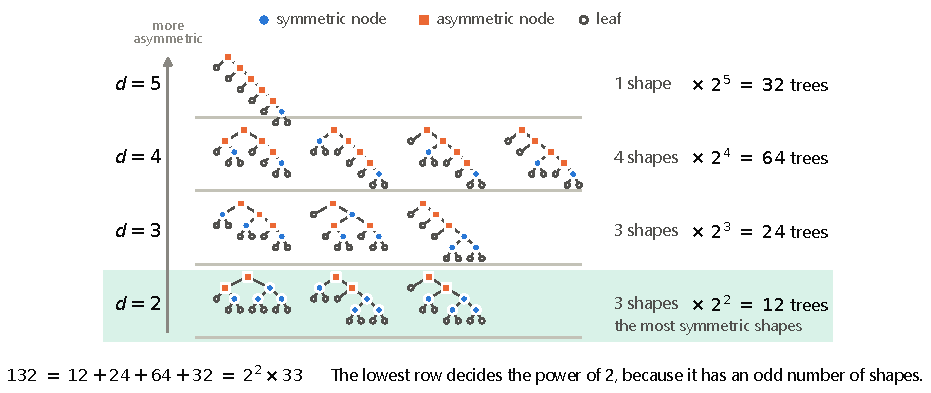
\includegraphics[width=0.93\textwidth]{figures/fig_levels.pdf}\\[2pt]
  \begin{minipage}{0.95\textwidth}\small
  For $2$-adic eyes $2^d$ is \emph{small} when $d$ is large, so the lowest row decides.
  A physicist would say: \textbf{the valuation is the ground-state energy}, and we must check that the number
  of ground states does not vanish modulo $p$. That is the shape of the proof.
  \end{minipage}
\end{frame}

\begin{frame}{Two more proofs \hfill\normalsize\textcolor{red!70!black}{checked by computer and by AI referees, not yet by us}}
  \textbf{Algebra only.} Trees by number of leaves: $G=x+G^q$.
  For every series, $f^p=f(x^p)+p\cdot\theta(f)$. Replace that $p$ by a variable $y$ (shown for $q=p$):
  \[ F=x+F(x^p,y^p)+y\,\theta(F). \]
  {\small $y$ marks asymmetric nodes.\quad $y=p$: ordered trees.\quad $y=1$: shapes.\quad
  $y=0$: only the complete trees, $x+x^p+x^{p^2}+\cdots$}\\[3pt]
  Digit sums give the lowest power $y^t$; a derivative identity modulo $p$ gives its coefficient.
  No tree, no formula for factorials; it shares no lemma with the main proof.

  \medskip
  \textbf{Accounting.} Label the leaves: each of the $\frac{m-1}{p-1}$ nodes is worth
  $-p$, and $m!$ absorbs $\frac{m-\sd(m)}{p-1}$ of them:\quad
  $\Cq\cdot\prod_j m_j!\equiv(-p)^{\,t}\pmod{p^{\,t+1}}$.
\end{frame}

% 15 -----------------------------------------------------------------
\begin{frame}{The idea in one sentence}
  \centering\Large
  Shrink the symmetry group until it is a $p$-group.\\[8pt]
  Then orbit sizes are powers of $p$,\\[4pt]
  the smallest orbits are built from the digits of $m$,\\[4pt]
  and a carry in base $p$ is a cherry collapsing.\\[14pt]
  \normalsize
  Exactness --- not just divisibility --- comes free.
\end{frame}

% 16 -----------------------------------------------------------------
\begin{frame}{How AI was used}
  \begin{itemize}
    \item \textbf{The idea and the proof sketch:} Claude Fable 5.2 (orchestrator).
    \item \textbf{Writing:} the full \LaTeX\ proof and these slides by Kimi K3.1 Pro
      (Open Math OS); independent re-check, literature scan, explainer and further
      drafts by other logged worker models (Mistral Large 4.0, Muse Spark Open,
      DeepSeek Flash).
    \item \textbf{Attacking:} three review rounds. Mistral Large 4.0, Muse Spark Open
      and a fresh Kimi K3.1 Pro found $14$ defects in the write-up; a line-by-line
      read by Claude found $4$ more; two further Claude referees who had seen none
      of our notes found $23$ smaller ones. No counterexample in any round; all
      repaired. Computer checks: every tree for small sizes, then $1067$ leaf counts
      up to $400$ leaves and primes up to $13$, no failures.
    \item \textbf{What humans verified:} \alert{to be filled in.}
  \end{itemize}
  \vfill
  {\small Full provenance: \texttt{JOURNAL.md}, \texttt{CLAIMS.md},
  \texttt{logs/delegations/} in the repository.}
\end{frame}

% 19 -----------------------------------------------------------------
\begin{frame}{What was known, and references}
  \footnotesize
  \begin{itemize}
    \item \textbf{$p=q=2$, exact valuation by orbits:} E.~Deutsch, B.~E.~Sagan,
      \emph{J.\ Number Theory} 117 (2006) 191--215. Weighted version: A.~Postnikov,
      B.~E.~Sagan, \emph{J.\ Combin.\ Theory Ser.\ A} 114 (2007) 970--977.
    \item \textbf{$q=p^k$, formula by factorials; divisibility by orbits of the full
      symmetric group:} M.~Konvalinka, \emph{J.\ Combin.\ Theory Ser.\ A} 114 (2007)
      1089--1100.
    \item \textbf{$p=2$, the minimal trees again, as most balanced evolutionary trees:}
      S.~J.~Kersting, M.~Fischer, \emph{Math.\ Biosci.} (2021),
      doi:10.1016/j.mbs.2021.108690. No mention of Catalan numbers.
    \item \textbf{Generating functions modulo prime powers, via $\sum z^{p^n}$:}
      M.~Kauers, C.~Krattenthaler, T.~W.~M\"uller, \emph{Electron.\ J.\ Combin.} 18(2)
      (2012) P37; C.~Krattenthaler, T.~W.~M\"uller, \emph{Aequationes Math.} 99 (2025)
      2505--2547. The starting point of our second, algebraic proof.
    \item \textbf{Counting trees up to a group at each node:} G.~P\'olya,
      \emph{Acta Math.} (1937). Sequences: OEIS A000625, A001190.
  \end{itemize}
  \medskip
  \textbf{Ours, as far as we could check:} the $p$-group action for $q=p^k$, the digit
  skeleton with its depth condition, the carry--cherry count, the residue for all
  prime powers. \emph{Not a certificate of novelty.}
\end{frame}

% ---- backup slides (added 2026-11-14) --------------------------------
\begin{frame}{Backup: a carry is two equal blocks fusing}
  \centering
  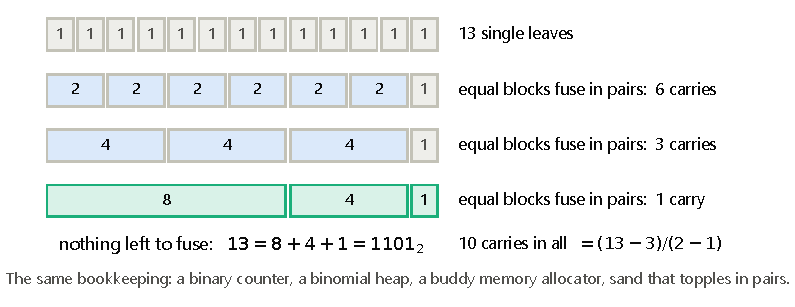
\includegraphics[width=0.95\textwidth]{figures/fig_fusion.pdf}\\[4pt]
  \begin{minipage}{0.93\textwidth}\small
  For a tree with $13$ leaves: $12$ nodes, at most $10$ of them symmetric (one per carry), so at least $2$
  asymmetric. In the proof, each fusion is a cherry of $p$ equal subtrees collapsing.
  \end{minipage}
\end{frame}

\begin{frame}{Backup: tree $=$ cut of an interval $=$ cut into balls}
  \centering
  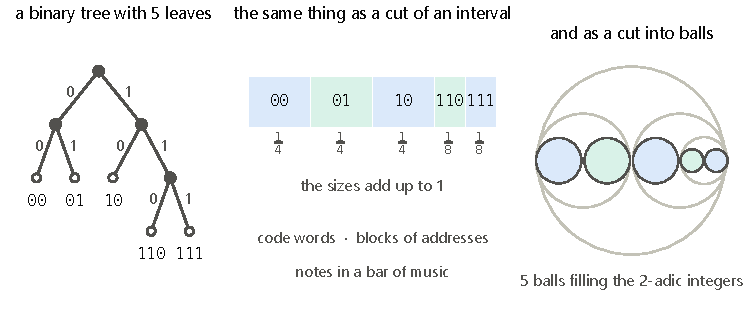
\includegraphics[width=0.95\textwidth]{figures/fig_balls.pdf}\\[4pt]
  \begin{minipage}{0.93\textwidth}\small
  The Catalan number $C_{m-1}$ counts the ways to cut the $2$-adic integers into $m$ balls; our rotations are
  isometries of them. In a computer the same cuts are prefix codes and blocks of addresses; for $q=2^8$ the
  blocks are aligned to whole bytes.
  \end{minipage}
\end{frame}

\begin{frame}{Backup: polymers ($p=3$)}
  \centering
  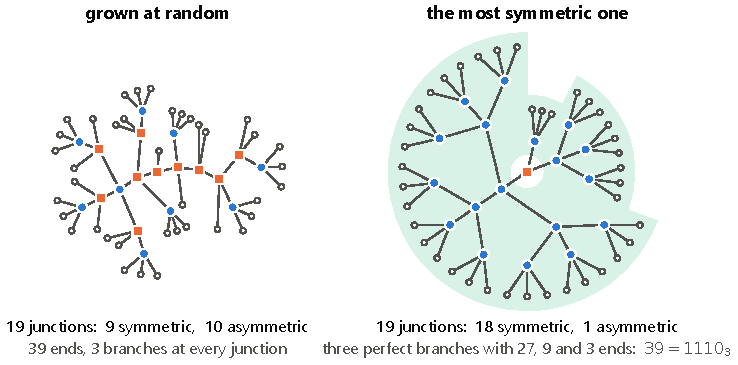
\includegraphics[width=0.8\textwidth]{figures/fig_dendrimer.pdf}\\[2pt]
  \begin{minipage}{0.95\textwidth}\small
  A molecule with $m$ ends can be perfectly branched only if $m$ is a power of $p$; otherwise it is $t$
  junctions short. Up to a simple factor, Fuss--Catalan numbers are the statistical weights of branched
  molecules in the classical theory of polymer branching (units with three reactive groups give the
  Catalan numbers).
  \end{minipage}
\end{frame}

\begin{frame}{Backup: prime powers as sand on a ring}
  \centering
  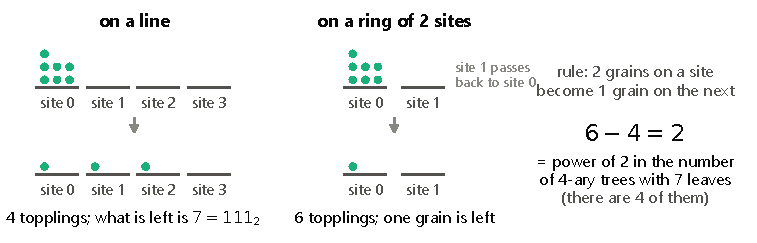
\includegraphics[width=0.92\textwidth]{figures/fig_sand.pdf}\\[4pt]
  \begin{minipage}{0.93\textwidth}\small
  For $q=p^k$: $p$ grains on a site topple into one grain on the next site, on a ring of $k$ sites.
  The power of $p$ in $\Cq$ is the number of topplings on the ring minus the number on a line.
  \end{minipage}
\end{frame}

\end{document}
